% VUT FIT MITAI
% MSZ 2021/2022
% Author: Vladimir Dusek
% Login: xdusek27

%%%%%%%%%%%%%%%%%%%%%%%%%%%%%%%%%%%%%%%%%%%%%%%%%%%%%%%%%%%%%%%%%%%%%%%%%%%%%%%%

% Path to figures
\graphicspath{{sui/prohledavani_stavoveho_prostoru/figures}}

%%%%%%%%%%%%%%%%%%%%%%%%%%%%%%%%%%%%%%%%%%%%%%%%%%%%%%%%%%%%%%%%%%%%%%%%%%%%%%%%

\chapter{SUI~--~Prohledávání stavového prostoru (informované a neinformované metody, lokální prohledávání, prohledávání v nejistém prostředí, hraní her, CSP úlohy).}

%%%%%%%%%%%%%%%%%%%%%%%%%%%%%%%%%%%%%%%%%%%%%%%%%%%%%%%%%%%%%%%%%%%%%%%%%%%%%%%%

\section{Zdroje}

\begin{compactitem}
    \item \path{opora_izu-esf-5a.pdf}
    \item \path{02-prohledavani.pdf}
    \item \path{03-lokalni_prohledavani.pdf}
    \item \path{04-prohledavani_nejiste_prostredi.pdf}
    \item \path{05-adversarial_search.pdf}
    \item \path{06-csp.pdf}
    \item \path{Wikipedia}
\end{compactitem}

%%%%%%%%%%%%%%%%%%%%%%%%%%%%%%%%%%%%%%%%%%%%%%%%%%%%%%%%%%%%%%%%%%%%%%%%%%%%%%%%

\section{Úvod a kontext}

\begin{compactitem}

    \item \textbf{Stavový prostor} je dvojice $(S, O)$, kde \begin{compactitem}
        \item $S = \{ s_1, s_2, \ldots, s_{n} \}$ je množina stavů (množina všech možných stavů úlohy).
        \item $O = \{ o_1, o_2, \ldots, o_{m} \}$ je množina operátorů (množina všech operátorů, kterými lze stavy úlohy měnit).
    \end{compactitem}

    \item \textbf{Úloha} je dvojice $(s_0, G)$, kde \begin{compactitem}
        \item $s_0 \in S$ je počáteční stav,
        \item $G = \{ s_{g1}, s_{g2}, \ldots \}$ je množina cílových stavů.
    \end{compactitem}

    \item \textbf{Řešení úlohy} je posloupnost operátorů:
    $$ s_1 = o_1(s_0), \ldots s_n = o_n(s_{n-1}) ~;~ s_n \in G $$
    \begin{compactitem}
        \item Řešení úlohy je nalezení sekvence akcí, které dosáhnou cíle.
    \end{compactitem}

    \item \textbf{Terminologie} \begin{compactitem}
        \item Expanze uzlu -- určení všech bezprostředních následovníků uzlu.
        \item Generace uzlu -- proces vytvoření uzlu.
    \end{compactitem}

    \item \textbf{Definice problému} \begin{compactenum}
        \item Počáteční stav.
        \item Množina akcí $a$, která lze provést v každém stavu $s$ ($a = getActions(s))$.
        \item Přechodový model, nový stav (deterministický) po provedení akce $a$ ze stavu $s$ -- $result(s, a)$.
        \item Test, je-li stav cílový -- $isGoal(s)$.
        \item Cena cesty (počet kroků v sekvenci).
    \end{compactenum}

    \item \textbf{Kritéria hodnocení algoritmů} \begin{compactitem}
        \item Úplnost -- Pokud nějaká řešení úlohy existují, tak úplná metoda jedno z nich musí nalézt.
        \item Optimálnost -- Pokud nějaká řešení úlohy existují, tak optimální metoda musí nalézt nejlepší z těchto řešení. Optimální metoda je vždy úplná.
        \item Časová složitost -- Jak dlouho trvá nalézt řešení.
        \item Paměťová složitost -- Kolik paměti je třeba pro nalezení řešení.
    \end{compactitem}

    \item \textbf{Známé úlohy} \begin{compactitem}
        \item Úloha dvou džbánů
        \item Úloha Loydovy osmičky
        \item Úloha osmi dam (CSP)
        \item Úloha hanojských věží
        \item Úloha balančních vah
        \item Problém barvení map (CSP)
    \end{compactitem}
\end{compactitem}

%%%%%%%%%%%%%%%%%%%%%%%%%%%%%%%%%%%%%%%%%%%%%%%%%%%%%%%%%%%%%%%%%%%%%%%%%%%%%%%%

\section{Neinformované metody pro prohledávání stavového prostoru}

\begin{compactitem}
    \item Algoritmy nevyužívají žádné další informace kromě samotné definice úlohy.

    \item Aby algoritmus pořád neopakoval stejné kroky, musí si svou historii nějak ukládat (seznam CLOSED).
\end{compactitem}

\subsection{Prohledávání do šířky (BFS -- Breadth First Search)}

\begin{compactitem}
    \item Prohledává postupně od nejbližších (vzdálenost chápeme jako počet uzlů na cestě).
    \item Používá FIFO frontu OPEN a seznam CLOSED.

    \item Hodnocení \begin{compactitem}
        \item Úplná, optimální (pokud jsou všechny akce stejně dobré -- fixní cena kroku).
        \item Časová a prostorová složitost: $\mathcal{O}(b^d)$.
    \end{compactitem}

    \begin{figure}[H]
        \centering
        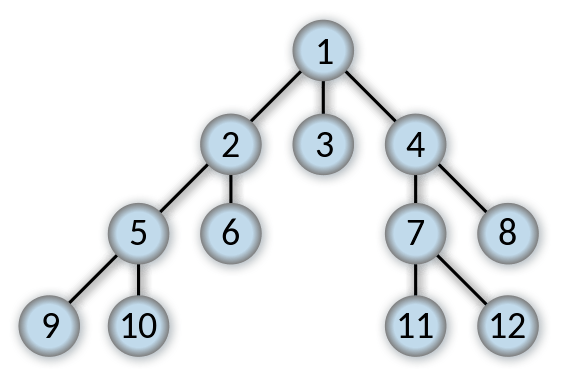
\includegraphics[width=0.5\linewidth]{bfs.png}
        \caption{Ukázka BFS. Pořadí, ve kterém jsou uzly expandovány odpovídá názvům uzlů.}
    \end{figure}
\end{compactitem}

\subsection{Uniform Cost Search (UCS, Best First Search)}

\begin{compactitem}
    \item De facto Dijkstrův algoritmus.
    \item Co když je každá akce jinak dobrá? \begin{compactitem}
        \item Stačí nevybrat nejbližší uzel (hloubka stromu), ale uzel s nejmenší cenou cesty.
        \item Slepé prohledávání do šířky s respektováním cen přechodů.
    \end{compactitem}

    \item Používá prioritní frontu OPEN a seznam CLOSED.

    \item Hodnocení \begin{compactitem}
        \item Úplná, optimální.
        \item Prostorová i časová složitost metody je dána cenou optimálního řešení ($C^*$) dělenou nejmenším přírůstkem ceny mezi dvěma uzly ($\Delta C_{min}$): $\mathcal{O}(b^{C^* / \Delta C_{min}})$.
    \end{compactitem}

    \begin{figure}[H]
        \centering
        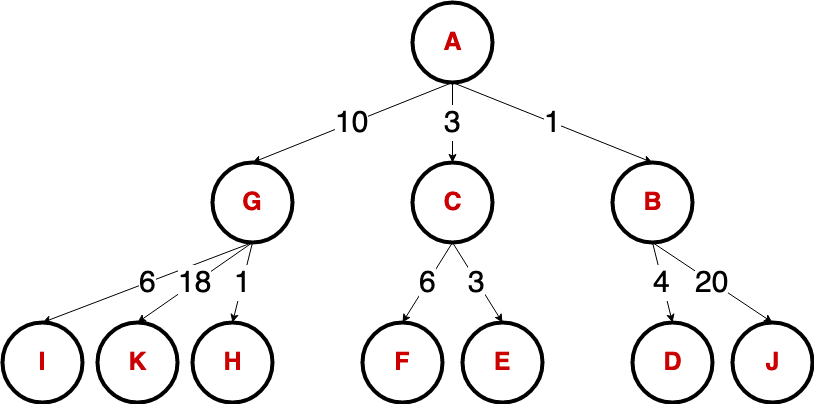
\includegraphics[width=0.6\linewidth]{ucs.png}
        \caption{Ukázka UCS. Pořadí, ve kterém jsou uzly expandovány odpovídá názvům uzlů.}
    \end{figure}
\end{compactitem}

\subsection{Prohledávání do hloubky (DFS -- Depth First Search)}

\begin{compactitem}
    \item DFS řeší problém s pamětí při prohledávání stromu (v grafu musíme stejně ukládat prozkoumané stavy, takže nám nepomůže).
    \item Používá LIFO zásobník OPEN a seznam CLOSED.

    \item Hodnocení \begin{compactitem}
        \item Není úplná, není optimální.
        \item Prostorová složitost: $\mathcal{O}(b \cdot m)$.
        \item Časová složitost: $\mathcal{O}(b^m)$.
    \end{compactitem}

    \item Vylepšení \begin{compactitem}
        \item Slepé prohledávání do omezené hloubky (Depth Limited Search - DLS).
        \item Slepé prohledávání do omezené hloubky s postupným zanořováním (Iterative Deeping Search - IDS) -- Postupně se volá procedura DLS a postupně se zvyšuje maximální hloubka.
    \end{compactitem}

    \begin{figure}[H]
        \centering
        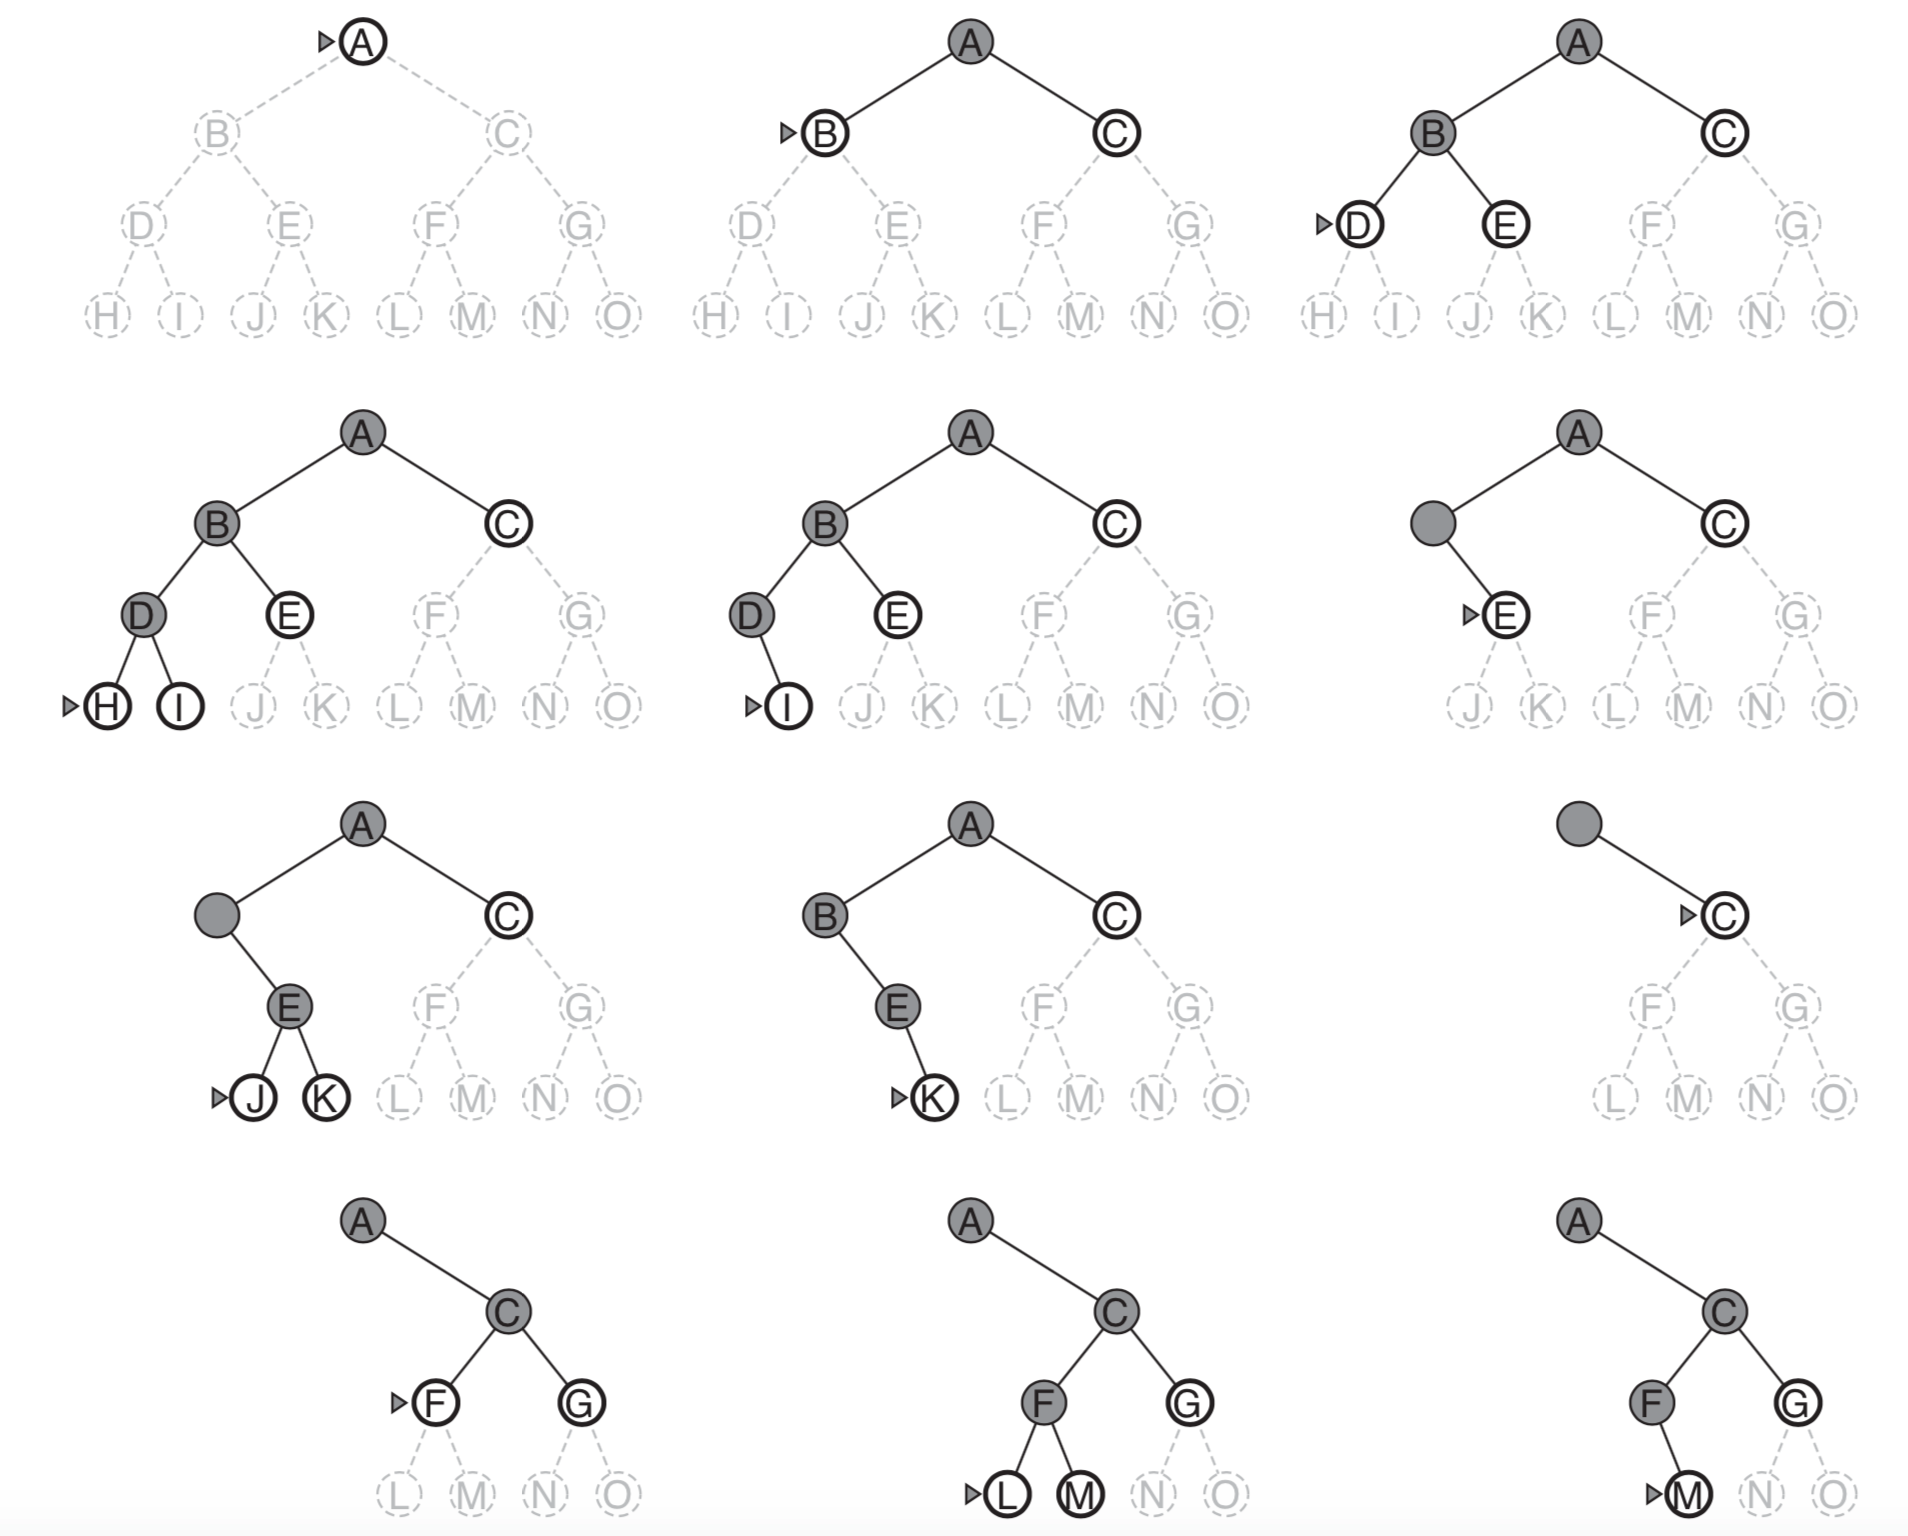
\includegraphics[width=1\linewidth]{dfs.png}
        \caption{Ukázka DFS.}
    \end{figure}
\end{compactitem}

\subsection{Prohledávání do omezené hloubky (DLS -- Depth Limited Search)}

\begin{compactitem}
    \item Vylepšení DFS, kde se omezí hloubka prohledávání. \begin{compactitem}
        \item Proč to dělat? Ochrana proti zacyklení.
    \end{compactitem}
    \item Úplná metoda, pokud není řešení ve větší
    hloubce, než je nastavený limit.
\end{compactitem}

\subsection{Prohledávání do omezené hloubky s postupným zanořováním (IDS -- Iterative Deeping Search)}

\begin{compactitem}
    \item Iterativní DLS, začíná se s limitem 0 a v každé iteraci se o 1 zvyšuje.
    \item Doporučená metoda při využití neinformovaných metod (pokud víme, že máme dostatek paměti, BFS bude rychlejší).
    \item Optimální metoda s malými paměťovými nároky.
    \item Optimálnost s ohledem na počet operací (ne cenu řešení).

    \begin{figure}[H]
        \centering
        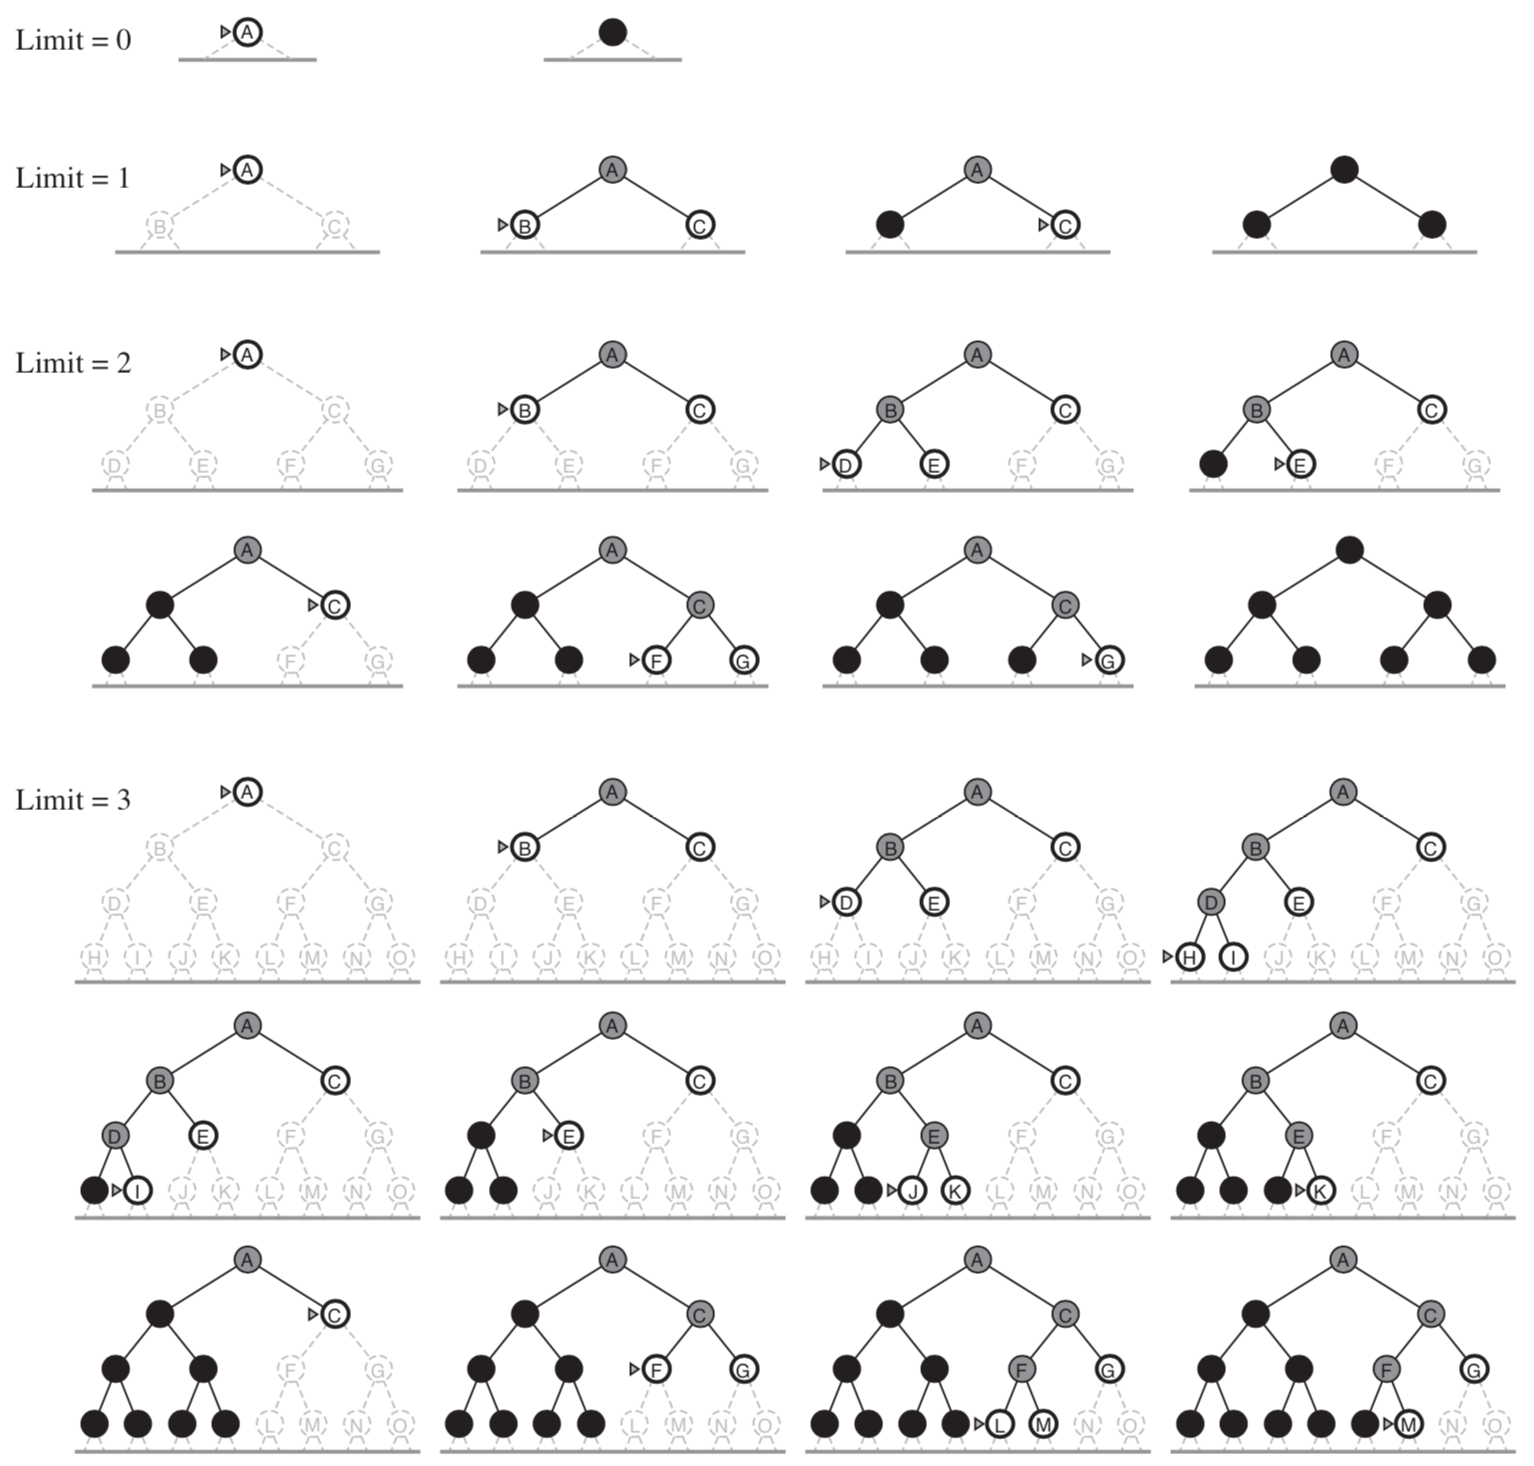
\includegraphics[width=1\linewidth]{ids.png}
        \caption{Ukázka IDS.}
    \end{figure}
\end{compactitem}

\subsection{Backtracking}

\begin{compactitem}
    \item Slepé prohledávání se zpětným návrácení \begin{compactitem}
        \item Operátory je nutné udržovat seřezené.
        \item Velmi podobné DFS, ale místo expanze uzlu (generování všech následníků) generuje pouze jediného následníka (nejprve prvního a při případných návratech další).
        \item Jde využít opět omezenou hloubku (jako u DLS).
    \end{compactitem}

    \item Využívá zásobník OPEN.

    \item Hodnocení \begin{compactitem}
        \item Není úplný, ani optimální.
        \item Extrémně nízká prostorová složitost.
    \end{compactitem}

    \begin{figure}[H]
        \centering
        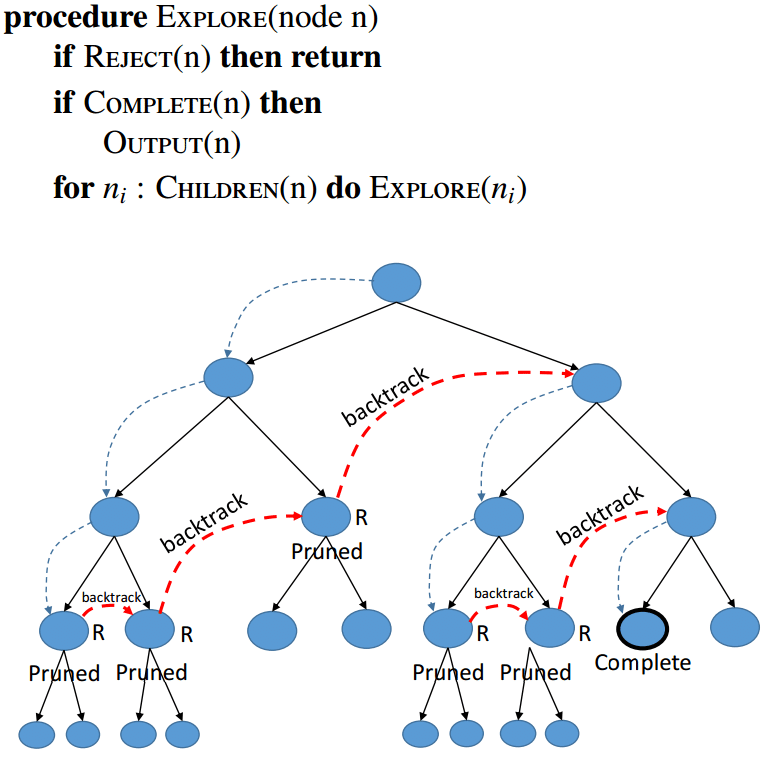
\includegraphics[width=1\linewidth]{backtracking.png}
        \caption{Ukázka Backtrackingu.}
    \end{figure}
\end{compactitem}

\subsection{Birectional Search (BS, obousměrné BFS)}

\begin{compactitem}
    \item BFS z počátečního a cílového stavu zároveň, hledá se spojení.
    \item Dá se použít pouze pro řešení úloh s reverzibilními operátory.
    \begin{compactitem}
        \item Např. lze použít pro řešení úlohy Loydovu osmičku, ale nelze použít pro řešení úlohy dvou džbánů.
    \end{compactitem}

    \item Hodnocení \begin{compactitem}
        \item Úplná, optimální.
        \item Časová a prostorová složitost: $\mathcal{O}(2b^{d / 2})$.
    \end{compactitem}

    \begin{figure}[H]
        \centering
        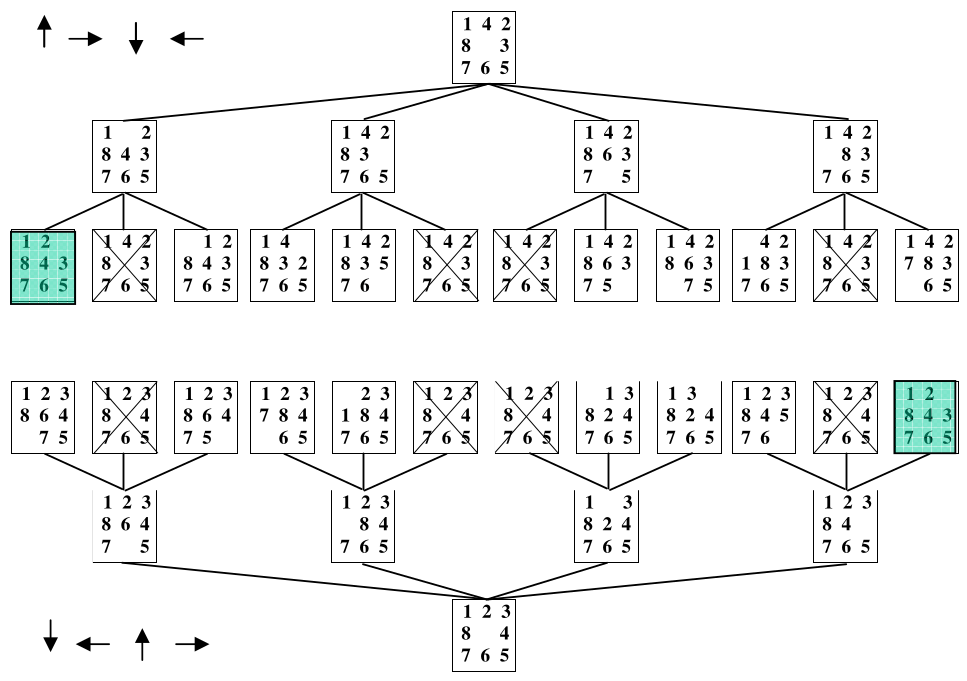
\includegraphics[width=1\linewidth]{bs.png}
        \caption{Ukázka BS, prohledávání stavového prostoru hlavolamu 8 metodou obousměrného prohledávání.}
    \end{figure}
\end{compactitem}

%%%%%%%%%%%%%%%%%%%%%%%%%%%%%%%%%%%%%%%%%%%%%%%%%%%%%%%%%%%%%%%%%%%%%%%%%%%%%%%%

\section{Informované metody pro prohledávání stavového prostoru}

\begin{compactitem}
    \item Algoritmy využívají informace o tom, jak je daný stav \uv{nadějný}.
    \item Implementace metod odpovídá UCS (jediná změna je způsob ohodnocení uzlů).
    \item UCS využíval pro ohodnocení uzlu $n$ funkci $g(n)$, která odpovídala nejkratší ceně cesty z počátečního uzlu do uzlu $n$.
    \item Informované metody se řídí podle funkce $f(n)$, která využívá funkci $h(n)$ a může mít tvar: \begin{compactitem}
        \item $f(n) = g(n) + h(n)$,
        \item $h(n)$ je heuristická funkce a je to odhad ceny cesty z uzlu $n$ do nejbližšího cílového uzlu.
    \end{compactitem}
\end{compactitem}

\subsection{Hladový algoritmus (Greedy Search)}

\begin{compactitem}
    \item \uv{Hladové/chamtivé prohledávání, bereme nejbližší krok.}

    \item Využívá se pouze heuristická funkce, $g(n) = 0$, $f(n) = h(n)$. \begin{compactitem}
        \item Odhadovanou cenou z daného uzlu do uzlu cílového.
        \item K expanzi vybírá uzel, který má toto hodnocení nejnižší.
        \item Např. vzdálenost vzdušnou čarou.
    \end{compactitem}

    \item Dobrá heuristika může časovou náročnost výrazně redukovat.

    \begin{figure}[H]
        \centering
        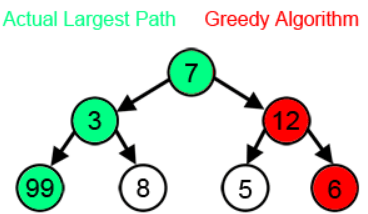
\includegraphics[width=0.5\linewidth]{greedy_search.png}
        \caption{Ukázka hladového algoritmu, vybírá maximum.}
    \end{figure}
\end{compactitem}

\subsection{A* Search}

\begin{compactitem}
    \item Využívají se obě složky funkce $f(n)$:
    $$ f(n) = g(n) + h(n) $$

    \item Úplná i optimální \begin{compactitem}
        \item Platí pro tzv. přípustné heuristiky, kdy odhad $h(n)$ nebude nikdy větší než reálná cena do cíle.
    \end{compactitem}

    \item Heuristika je v tomto případě chápána jako způsob prořezávání (prunning) -- vyloučení některých možností bez jejich prozkoumání.

    \begin{figure}[H]
        \centering
        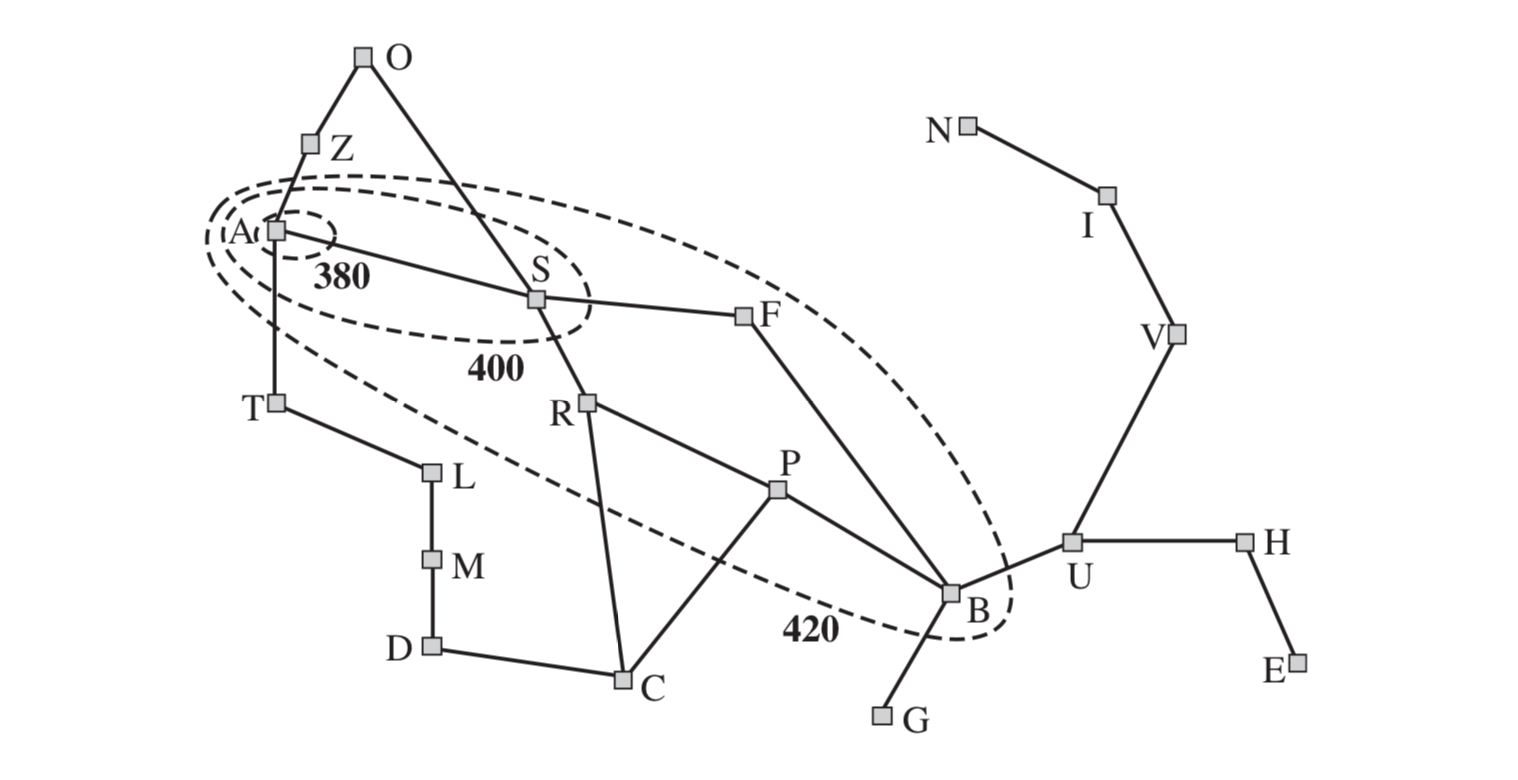
\includegraphics[width=1\linewidth]{a_star.png}
        \caption{Ukázka A* Search.}
    \end{figure}
\end{compactitem}

%%%%%%%%%%%%%%%%%%%%%%%%%%%%%%%%%%%%%%%%%%%%%%%%%%%%%%%%%%%%%%%%%%%%%%%%%%%%%%%%

\section{Lokální prohledávání}

\begin{compactitem}
    \item Neprohledáváme systematicky celý prostor, jsme pouze v jednom (nebo i více) aktuálním uzlu (stavu), který vyhodnocujeme a modifikujeme.

    \item Metody využívají málo paměti, jsou použitelné pro řešení úloh ve velkých (i spojitých) prostorech, kde nemáme zdroje pro prozkoumání všech možností.

    \item Abychom získali nový uzel ze současného, využíváme sousednost uzlů (např. skrze akce, náhodná malá změna, kombinace více uzlů).
\end{compactitem}

\subsection{Hill climbing}

\begin{compactitem}
    \item Také označovaný jako \textit{greedy local search}.

    \item Jako nový uzel se zvolí nejlepší ze sousedních uzlů (steepest-ascent varianta), který je zároveň lepší než současný uzel; pokud takový není, výsledným řešením (výstupem algoritmu) je současný uzel.

    \item Problematické jsou lokální extrémy a části, na kterých je funkce konstantní (plateau).

    \item Gradient descent u trénování neuronových sítí by sem spadal (resp. varianta tohoto algoritmu pro spojité prostředí).

    \item Vylepšení: \begin{compactitem}
        \item Stochastic hill climbing -- pokud je více sousedních uzlů lepších než aktuální, nemusí se volit ten nejlepší.

        \item Random-restart hill climbing -- jeden běh algoritmu nalezne lokální extrém, pokud iterativně spouštíme algoritmus s (náhodnou) inicializací, zvyšujeme pravděpodobnost nalezení globálního extrému.
    \end{compactitem}

    \begin{figure}[H]
        \centering
        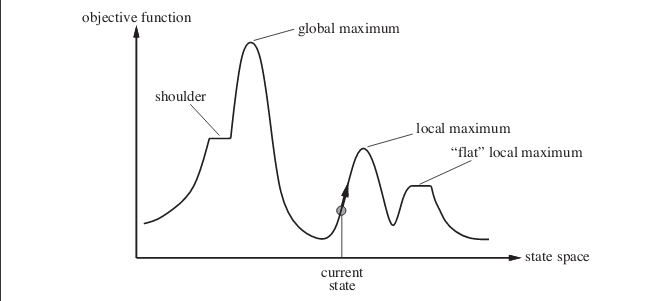
\includegraphics[width=1\linewidth]{hill_climb_searching.png}
        \caption{Ukázka Hill climbing.}
    \end{figure}
\end{compactitem}

\subsection{Simulated annealing}

\begin{compactitem}
    \item Kombinace hill-climbing a náhodné procházky (volíme náhodného souseda).
    \item Náhodně vybíráme sousední uzel, pokud je lepší než současný, nahradíme, pokud je horší, spočítáme, o kolik je horší $\Delta E$ (záporné číslo).
    \item Myšlenka snižování teploty $T$ v každé iteraci (čím nižší je teplota, tím menší pravděpodobnost nahrazení horším uzlem).
    \item Pravděpodobnost nahrazení horším uzlem se spočítá podle vztahu $e^{\Delta E / T}$.

    \begin{figure}[H]
        \centering
        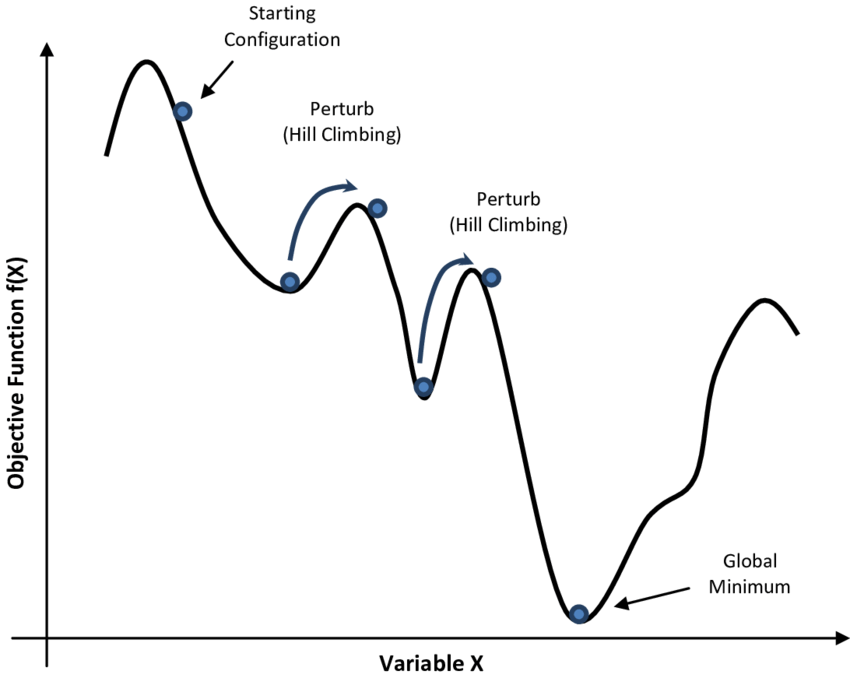
\includegraphics[width=1\linewidth]{simulated_annealing.png}
        \caption{Ukázka Simulated annealing.}
    \end{figure}
\end{compactitem}

% \subsection{Local beam search}

% \begin{compactitem}
%     \item Vychází z beam search -- princip je podobný BFS, ale uchováváme pouze omezené množství uzlů. \begin{compactitem}
%         \item Nejprve expandujeme počáteční uzel, ponecháme však pouze $k$ nejlepších následníků, pak expandujeme těchto $k$ následníků, z nichž ponecháme opět $k$ nejlepších atd.
%     \end{compactitem}

%     \item Local beam search můžeme chápat jako beam search inicializovaný několika počátečními uzly.
% \end{compactitem}

% \subsection{Genetický algoritmus}

% \begin{compactitem}
%     \item Nejprve se selekcí vyberou rodiče, pak se křížením vytvoří potomci a následně v některých případech dochází k mutaci, nakonec se upraví původní populace a proces se opakuje. \begin{compactitem}
%         \item Fitness funkce -- vyhodnocovací metrika (objektivní funkce) u GA.
%         \item Selection (selekce) -- výběr rodičů.
%         \item Crossover (křížení) -- proces vytvoření nového potomka z rodičovských uzlů.
%         \item Mutation (mutace) -- náhodná změna potomka.
%     \end{compactitem}
% \end{compactitem}

%%%%%%%%%%%%%%%%%%%%%%%%%%%%%%%%%%%%%%%%%%%%%%%%%%%%%%%%%%%%%%%%%%%%%%%%%%%%%%%%

\section{Prohledávání v nejistém prostředí}

\begin{compactitem}
    \item Máme nedeterministické akce (nejisté prostředí, částečně pozorovatelné prostředí).

    \item Zadaný problém již nelze řešit pouze pevně danou sekvencí akcí, ale potřebujeme vytvořit nějaký plán / strategii.

    \item Výsledkem $RESULT(s, a)$ je nyní množina akcí a
    cena $COST(s, a, s')$ provedení akce $a$ ve stavu $s$ závisí také na novém stavu $s'$, ve kterém se ocitneme po provedení akce.

    \item Dříve jsme věděli, co se stane po provedení akce, plán = sekvence akcí (nezávisle na vjemech) Nyní se rozhodujeme i na základě vjemů.

    \item Řešení pomocí AND / OR prohledávacích stromů (operátor and se používá pro výsledek nedeterministické akce). \begin{compactitem}
        \item OR -- můžu si vybrat, kterou akci provedu.
        \item AND -- výsledkem akce může být více stavů, řešení pro všechny možné nové stavy.
    \end{compactitem}

    \begin{figure}[H]
        \centering
        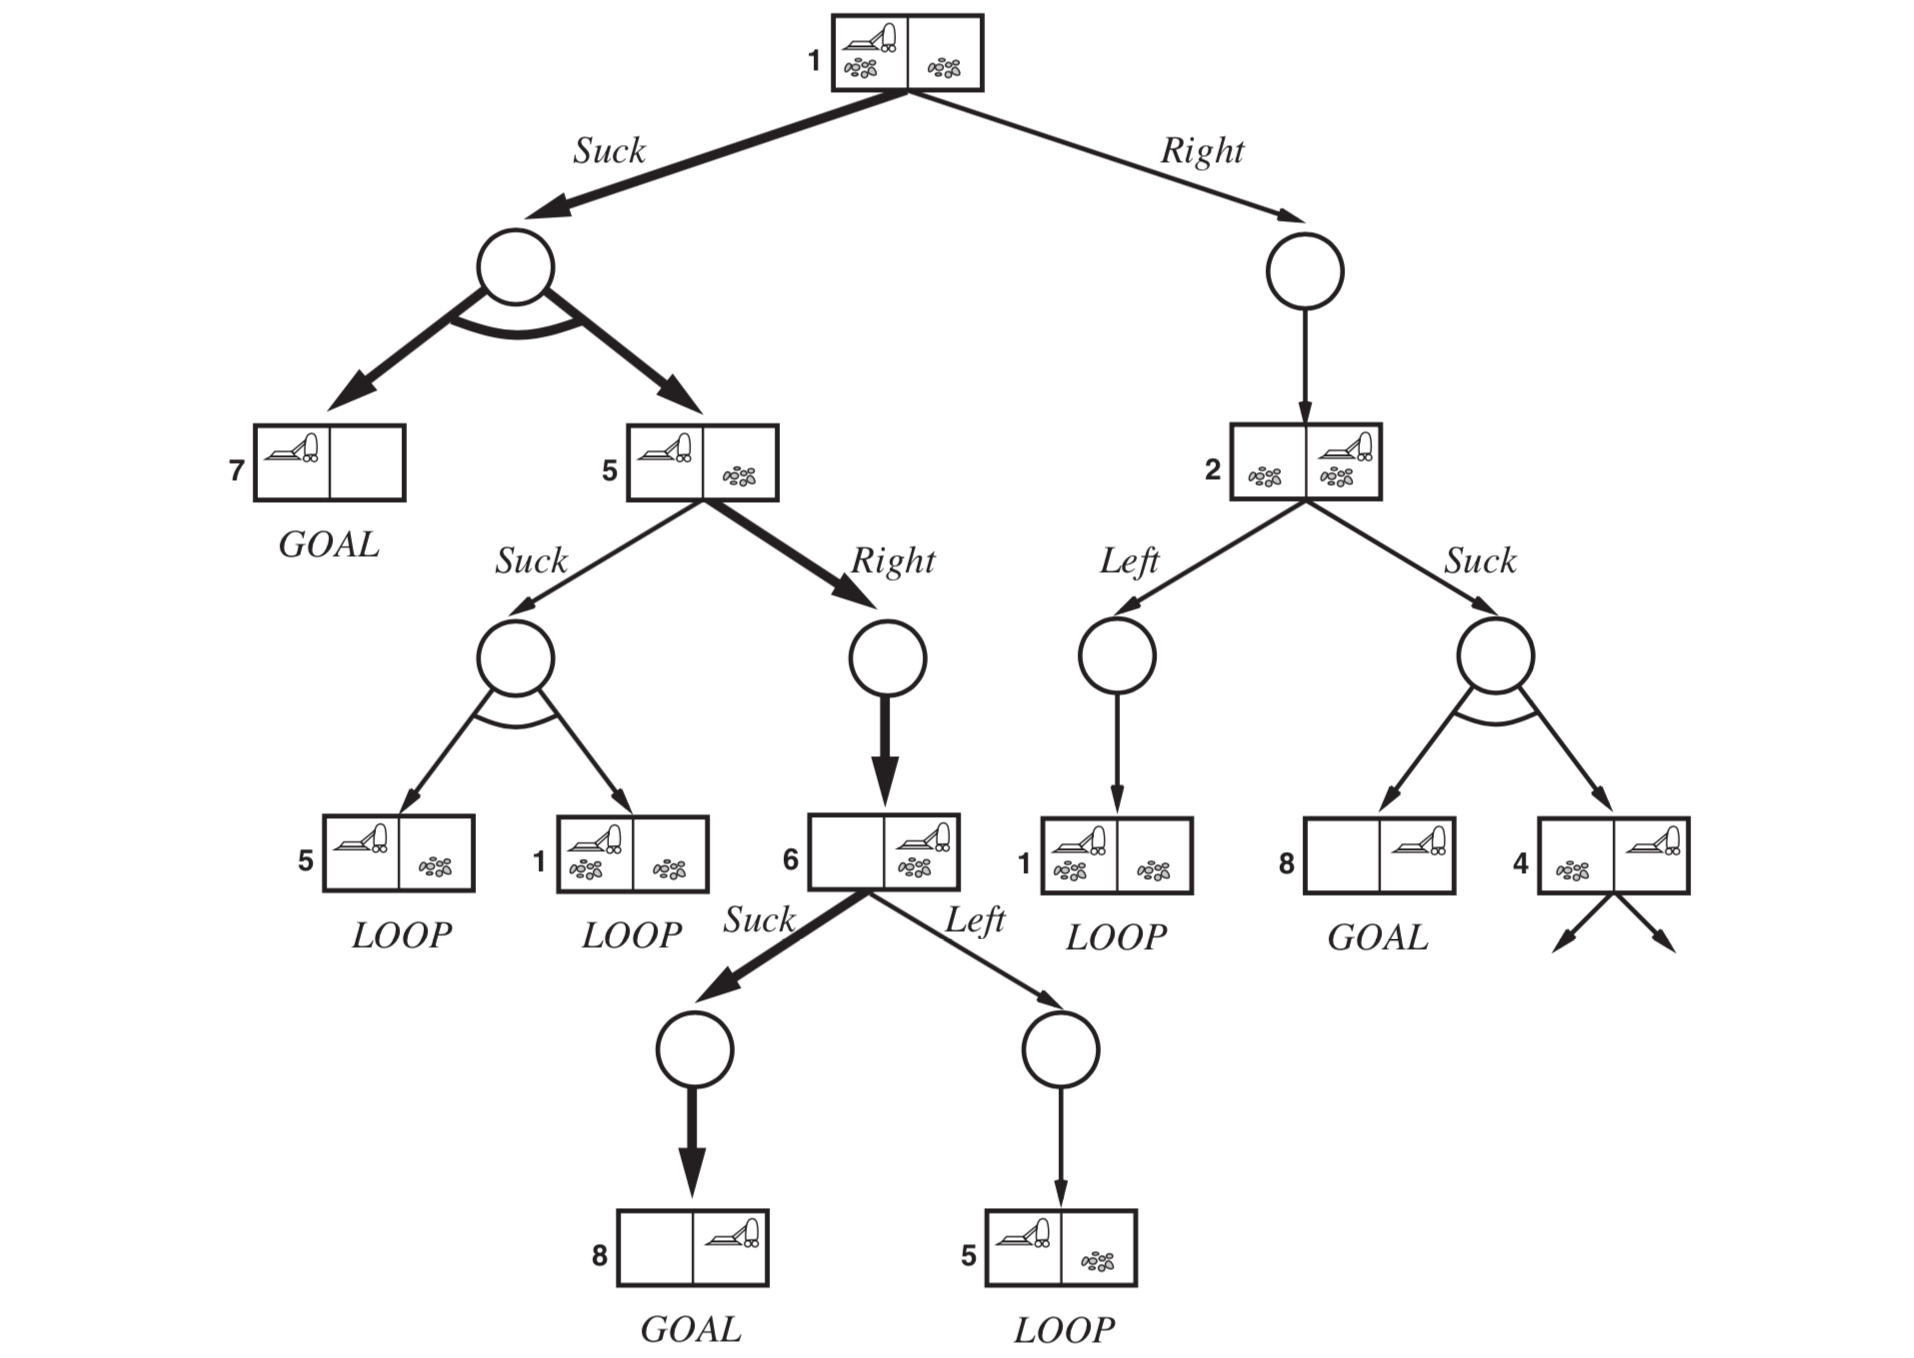
\includegraphics[width=1\linewidth]{and_or_prohledavaci_stromy.png}
        \caption{AND-OR prohledávací stromy.}
    \end{figure}

    \item Bavíme se o belief state -- reflektuje agentovu důvěru o aktuálním stavu (v jakých stavech se může nacházet). V nepozorovatelném prostředí se vyskytuje celkem $2^n$ belief states.

    \item Incremental belief-state search -- postupně hledáme řešení pro každý stav; výhoda: pokud neexistuje řešení, zjistí se rychle; jiná řešení později. Udržování si Belief state je základem inteligentního agenta v ČPP (většina reálných prostředí).

    \begin{figure}[H]
        \centering
        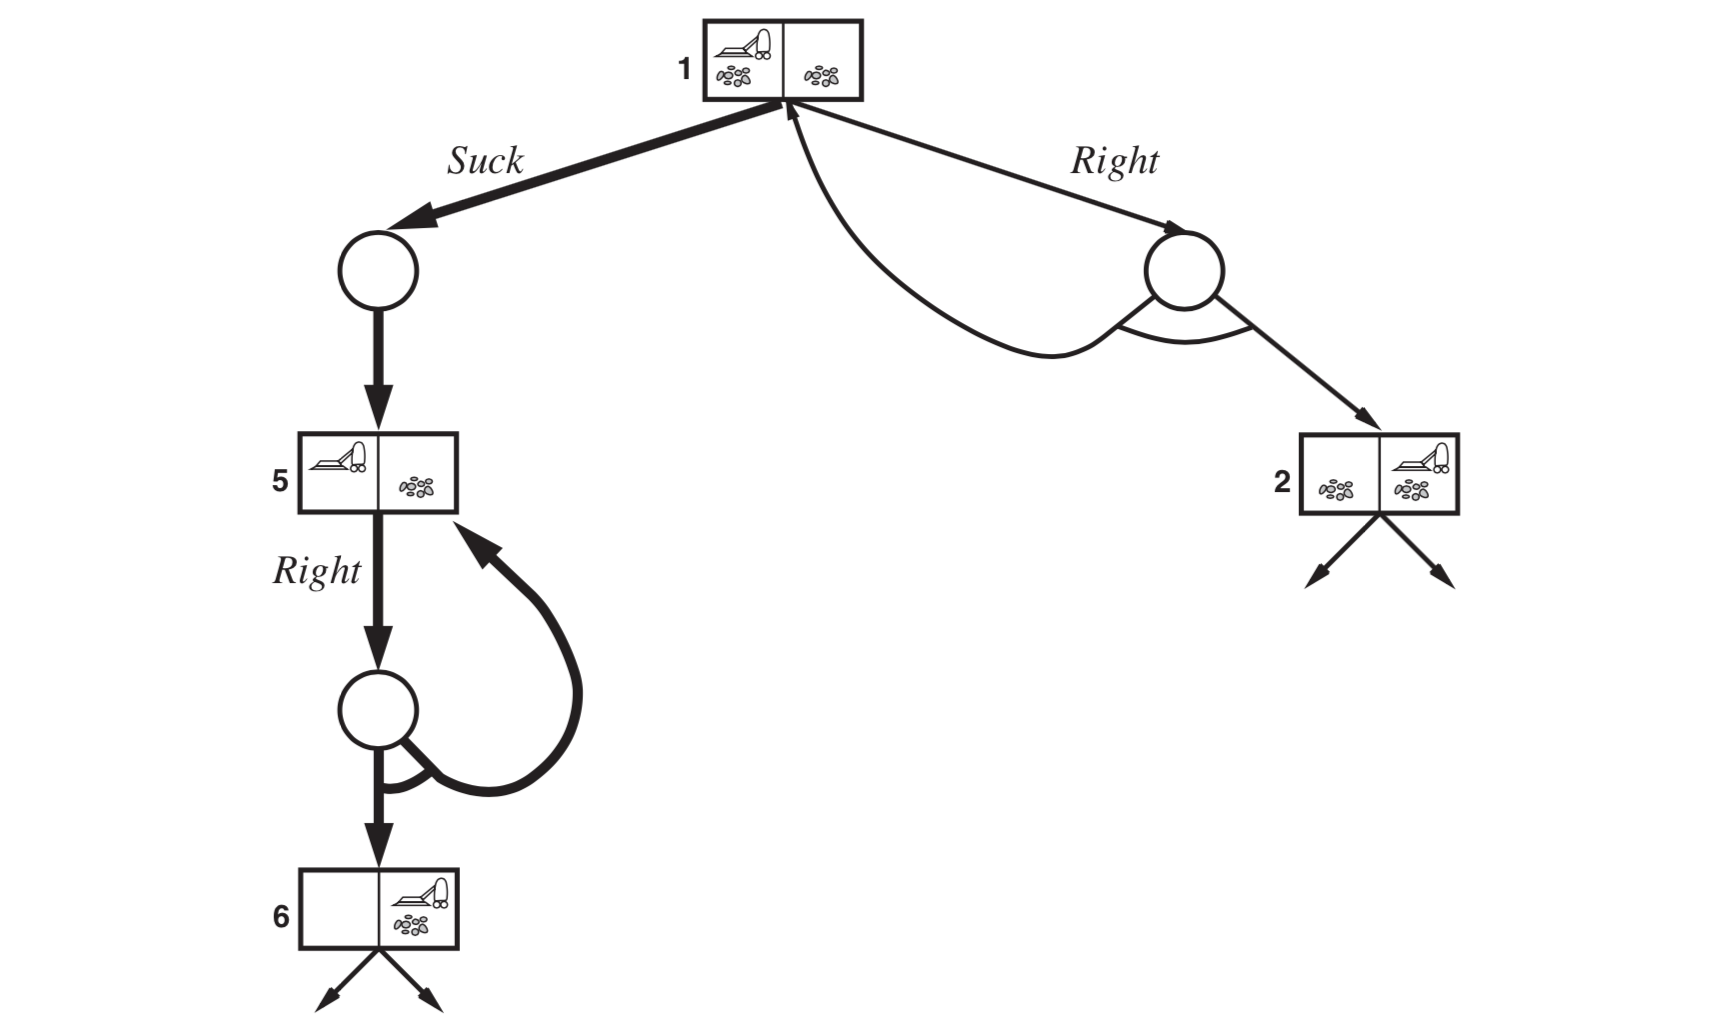
\includegraphics[width=1\linewidth]{nedeterministicke_akce.png}
        \caption{Nedeterministické akce: pohyb může selhat.}
    \end{figure}
\end{compactitem}

%%%%%%%%%%%%%%%%%%%%%%%%%%%%%%%%%%%%%%%%%%%%%%%%%%%%%%%%%%%%%%%%%%%%%%%%%%%%%%%%

\section{Hraní her (adversial search)}

\begin{compactitem}
    \item Typ prohledávání v soutěživém prostředí, často ho označujeme jako hry teorie her (game theory).

    \item Nejčastěji se jedná o speciální druh her: \begin{compactitem}
        \item Hry s nulovým součtem (zero-sum game) -- Součet zisku/užitku všech hráčů je konstantní -- typ her, ve kterých není možné, aby všichni prosperovali (lepší výsledek je na úkor druhých).
        \item Tahové
        \item Dvou hráčů
        \item Perfect information (plně pozorovatelné)
        \item Deterministické
    \end{compactitem}

    \item Multiagentní prostředí, pokud se v prostředí vyskytují dva agenti, chápeme to tak, že nám druhý agent (hráč) chce škodit.

    \item Prozkoumat všechny možnosti je u většiny her (stejně jako rozhodování v reálném světě) nemožné a přesto nutné zvolit nějakou akci (tah).

    \item Hra má svůj strom (game tree), my ovšem prohledáváme pouze některé části tohoto stromu, což je náš prohledávací strom (search tree).

    \item Každý stav hry je ohodnocen hodnotící funkcí. Kladné hodnoty této funkce musí znamenat příznivý stav pro hráče na tahu (hráče A). Záporné pak příznivý stav pro protihráče (hráče B).
\end{compactitem}

\subsection{Algoritmus MiniMax}

\begin{compactitem}
    \item Hry dvou hráčů.
    \item Racionální chování, protivník vždy zvolí svůj nejlepší tah (pro nás nejhorší).

    \begin{figure}[H]
        \centering
        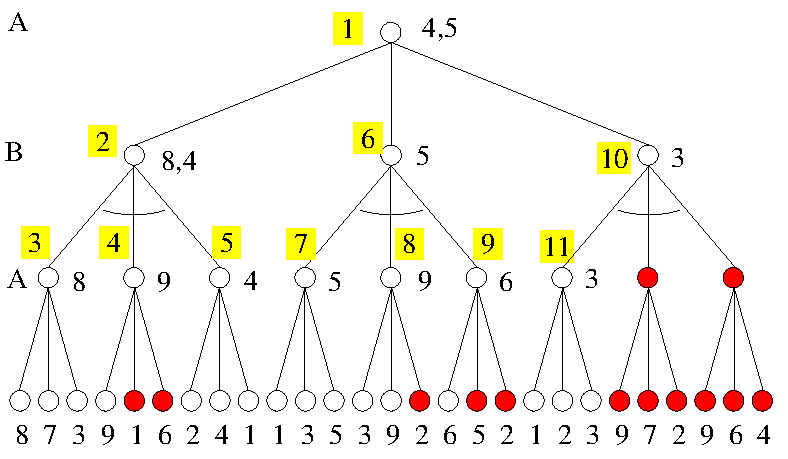
\includegraphics[width=1\linewidth]{mini_max.pdf}
        \caption{Příklad na zbytečná vyšetřování některých uzlů AND/OR grafu metodou MiniMax.}
    \end{figure}
\end{compactitem}

\subsection{Alpha-beta pruning}

\begin{compactitem}
    \item Hry dvou hráčů.
    \item Stejné jako MiniMax ale používá pruning.
    \item Alpha -- dosavadní nejlepší tah pro MAX
    \item Beta -- dosavadní nejlepší tah pro MIN
    \item Neprohledávat zbytečně, pokud by MIN nebo MAX tento tah stejně neprovedli.

    \begin{figure}[H]
        \centering
        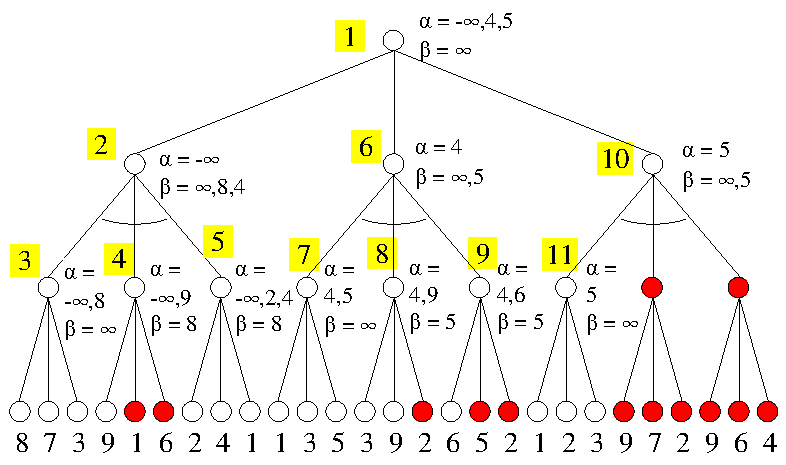
\includegraphics[width=1\linewidth]{alpha_beta.pdf}
        \caption{Příklad práce procedury AlfaBeta (alfa a beta řezů).}
    \end{figure}
\end{compactitem}

%%%%%%%%%%%%%%%%%%%%%%%%%%%%%%%%%%%%%%%%%%%%%%%%%%%%%%%%%%%%%%%%%%%%%%%%%%%%%%%%

\section{Úlohy s omezujícíma podmínkama}

\begin{compactitem}
    \item Úlohy s omezujícíma podmínkama (CSP, \textit{constraint satisfaction problem}).

    \item Záleží pouze na nalezení cílového stavu při splnění předem daných omezujících podmínek (není důležitý postup!).

    \item Stavy v CSPs jsou obvykle definovány množinou proměnných, kterým se přiřazují hodnoty z množin přípustných hodnot pro tyto proměnné.

    \item Opět nehledáme sekvenci akcí/tahů, nyní se ani nesnažíme najít nejlepší řešení. Hledáme pouze nějaké řešení, které splňuje předem stanovené podmínky pro kombinaci hodnot proměnných.

    \item Formální definice CSP úlohy: \begin{compactitem}
        \item $X$ je množina proměnných,
        \item $D$ je množina domén,
        \item $D_i$ je domána pro $X_i$,
        \item $C$ je množina omezení, která definují povolené kombinace hodnot.
    \end{compactitem}

    \item \textbf{Naivní prohledávání} v každé úrovni stromu přiřadí hodnotu jedné proměnné, po přiřazení všech se zkoumá, jestli je řešení konzistentní.

    \item \textbf{Inference je alternativa} k prohledávání. Uvažujeme inferenci nazývanou constraint propagation CP. Snahou je snížit počet hodnot v
    doménách, což zrychlí prohledávání. Existuje několik algoritmů využívajících tento přístup.
\end{compactitem}

\subsection{Backtracking pro CSP}

\begin{compactitem}
    \item Metodu zpětného navracení (backtracking) lze k řešení CSP použít velmi snadno -- pokud aplikace operátoru vede na stav porušující omezující podmínky, pak je tento operátor považován za neaplikovatelný a vrací se o krok zpět.

    \item Metoda je úplná (a každá úplná metoda je pro CSP optimální). Označíme-li symbolem $n$ počet proměnných a symbolem $m$ maximální počet přiřaditelných hodnot, pak platí: \begin{compactitem}
        \item Pro prostorovou složitost: $\mathcal{O}(n)$
        \item Pro časovou složitost: $\mathcal{O}(m^n)$
    \end{compactitem}

    \begin{figure}[H]
        \centering
        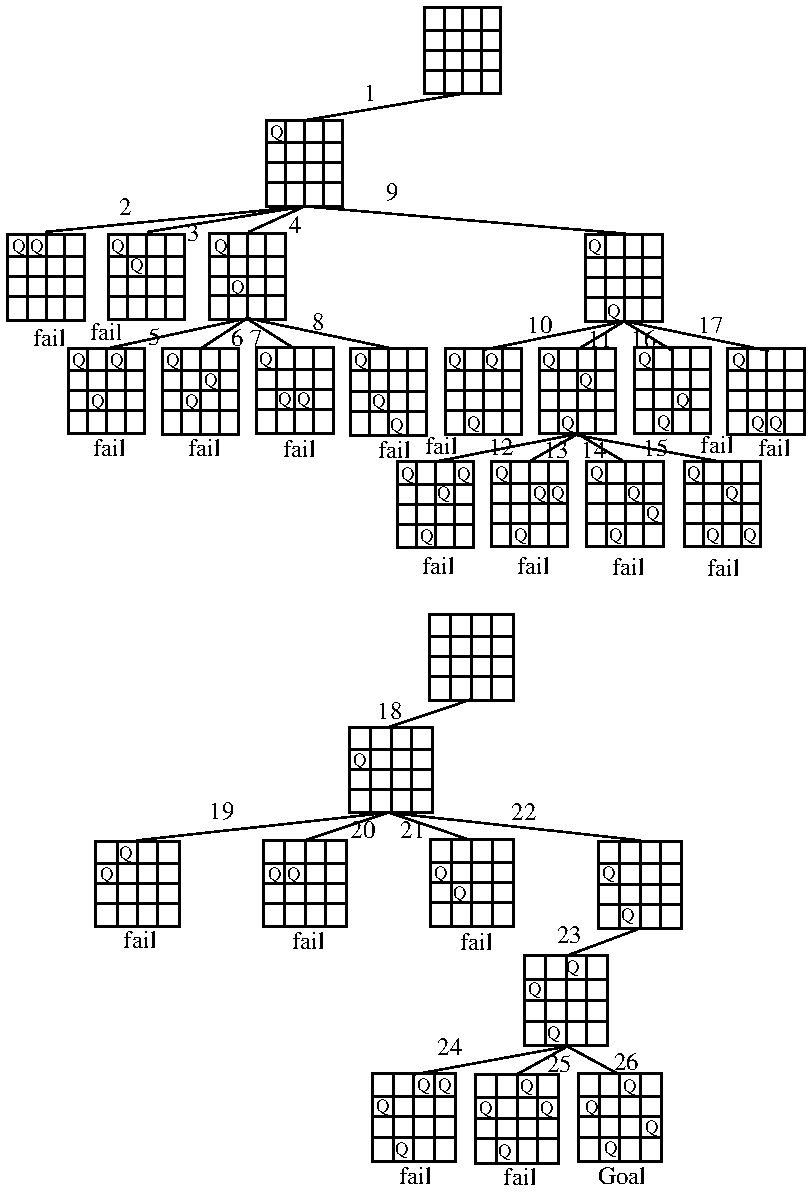
\includegraphics[width=1\linewidth]{backtrack_csp.pdf}
        \caption{Řešení úlohy čtyř dam metodou Backtracking for CSP (fail značí neúspěch, Goal znamená cíl).}
    \end{figure}
\end{compactitem}

\subsection{Forward-checking}

\begin{compactitem}
    \item Princip algoritmu Forward checking spočívá v tom, že po každém přiřazení hodnoty nějaké proměnné vyřazuje z množin přípustných hodnot dosud volných proměnných ty hodnoty, které jsou s právě přiřazenou hodnotou v konfliktu.

    % \item Algoritmus je dán procedurou, která rekurzivně volá sama sebe: \begin{compactitem}
    %     \item Přiřaď každé proměnné $i = 1, 2, \ldots, n)$ množinu přípustných hodnot $S_i$.
    %     \item Volej proceduru $Forward\_Checking$ pro první proměnnou $(i = 1)$.
    % \end{compactitem}

    \begin{figure}[H]
        \centering
        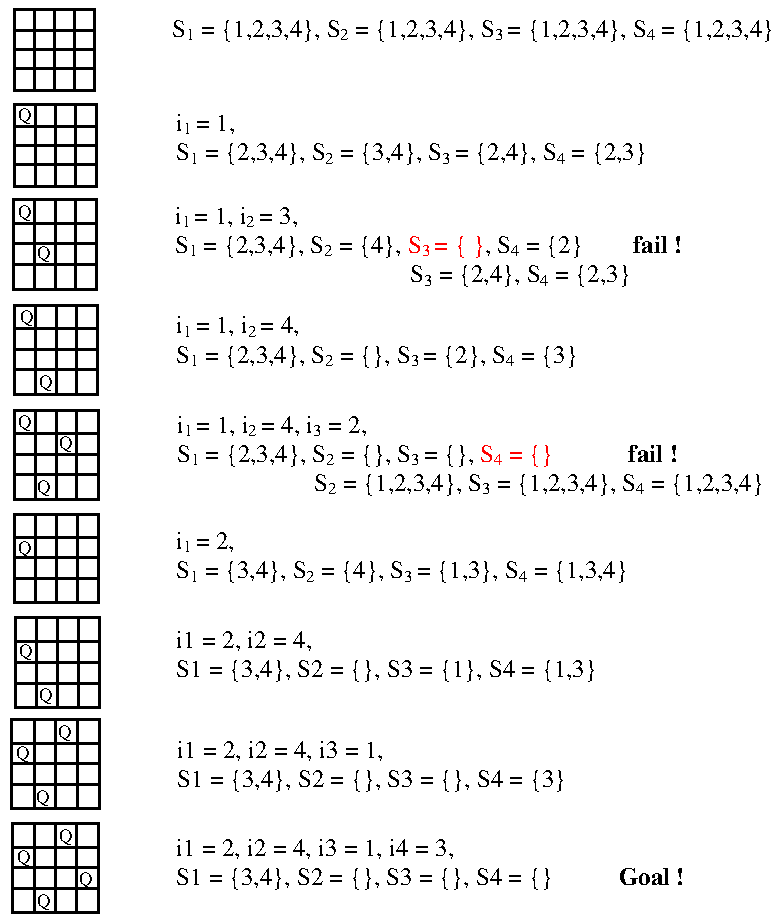
\includegraphics[width=1\linewidth]{forwardcheck_csp.pdf}
        \caption{Řešení úlohy čtyř dam metodou Forward checking (fail značí neúspěch, Goal znamená cíl).}
    \end{figure}
\end{compactitem}
